
\section{Experiments}\label{sec:experiments}
\newcommand{\TO}{\multicolumn{1}{r|}{TO}}
\newcommand{\TI}{\multicolumn{1}{r|}{T}}

Our approach aims at a simple yet general framework for incorporating theory reasoning into ASP solving.
Hence, it leaves room for various ways of encoding a problem and of implementing theory propagation.
%
To reflect this from a practical perspective,
we empirically explore several options for solving problems with difference logic (\DL) constraints.
%
To be more precise,
we contrast an encoding relying on \emph{defined} theory atoms with one leaving them \emph{external} (cf.\ Section~\ref{sec:foundations}),
and a \emph{stateless} with a \emph{stateful} propagator implementation.
As a \emph{non-strict} interpretation of \DL\ constraints is sufficient
for the problems given below,
we stick to this option and do not vary it.

The consistency of a set $C$ of \DL\ constraints can be checked by mapping them to a weighted directed graph $G(C)$.
The nodes of $G(C)$ are the (integer) variables occurring in $C$,
and for each $x_1 - x_2 \leq k$ in $C$, $G(C)$ includes an edge from $x_1$ to $x_2$ with weight $k$.
Then, $C$ is \DL-consistent iff $G(C)$ contains no cycle whose sum of edge weights is negative.
%
The difference between a stateless and stateful \DL-propagator amounts to whether the corresponding graph is
built from scratch upon each invocation or only once and updated subsequently.
%
In our experiments,
we use the Bellman-Ford algorithm \cite{bellman58a,forful62a} as basis for a stateless propagator,
and the one in \cite{cotmal06a} for update operations in the stateful case.
%
Both propagator implementations detect negative cycles
and record (solver) literals corresponding to their weighted edges as nogoods.

Theory atoms corresponding to \DL\ constraints are formed as described in Section~\ref{sec:language}.
%
The difference between using defined and external theory atoms boils down to their occurrence in the head of a rule,
as in Line~\ref{prg:diff:rule-diff} of Listing~\ref{prg:diff}, viz.\
\begin{lstlisting}[morekeywords={&diff},alsoletter={\&},numbers=none]
&diff { end(T)-start(T) } <= D :- duration(T,D).
\end{lstlisting}
or in the body, as in
\begin{lstlisting}[morekeywords={&diff},alsoletter={\&},numbers=none]
:- duration(T,D), not &diff { end(T)-start(T) } <= D.
\end{lstlisting}
% Although we cannot detail the full encoding,
Note that the defining usage constrains \DL-atoms firmer than the external one:
A defined \DL-atom is true iff at least one of its bodies holds,
while an external one may vary whenever its truth is \DL-consistent yet
not imposed by integrity constraints (with further problem-specific literals).
% while external theory atoms may also be true if atoms in the integrity constraint are false.
% This allows defined theory atoms to avoid symmetric solutions\comment{BK: Sentence does not sound right to me}.

To evaluate the different options,
we expressed (decision versions of) several scheduling problems \cite{taillard93a},
typically aiming at the minimization of schedules' makespan,
by logic programs in the language of Section~\ref{sec:language}.
% More precisely,
% we consider the following benchmarks.
%
\emph{Flow shop}:
A schedule corresponds to a permutation of~$n$ jobs,
each including $m$ sequential subtasks allocating
machines $1,\dots, m$ for specific amounts of time.
% that have to be executed on $m$ machines (while minimizing the makespan);
% each job has to be assigned to the machines in order $1\dots m$;
% and the job order is the same on all machines.
%
\emph{Job shop}:
Again considering~$n$ jobs with $m$ sequential subtasks each,
where the order in which subtasks allocate machines $1,\dots, m$ for given amounts of time
is job-specific,
a schedule arranges the subtasks of different jobs in one sequence per machine.
% $n$ jobs have to be placed on $m$ machines (so that the \REP{make-span}{makespan} is minimal);
% each job has an assigned sequence in which it has to be scheduled on the machines;
% the order of jobs on machines may differ.
%
\emph{Open shop}:
Given the same setting as in the job shop problem,
the sequential order of the subtasks of a job is not fixed,
but augments a schedule arranging the subtasks of different jobs per machine.
% $n$ jobs have to be placed on $m$ machines (so that the \REP{make-span}{makespan} is minimal);
% as job shop but the sequence of jobs on different machines may be arbitrary;
% a job cannot be executed on two machines simultaneously.
%
For reasons of scalability,
we refrain from optimizing the makespan of schedules,
but are only interested in some feasible schedule per instance along with
the corresponding earliest start times of subtasks.

\begin{table}
\caption{Comparison between different encodings and \DL-propagators for scheduling problems}
\centering
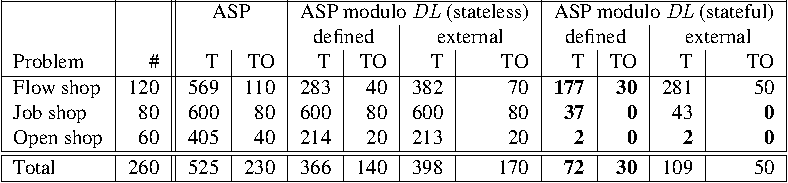
\includegraphics{tables/shop-scheduling}
\label{table:bench:encoding_comparisson}
\end{table}
The results of our experiments,
run sequentially under Linux on an Intel Xeon E5520 2.27~GHz machine equipped with 24~GB main memory,
are summarized in Table~\ref{table:bench:encoding_comparisson}.
%
% They were obtained on an Intel Xeon E5520 with 8x2.27~GHz CPU and 24~GB of memory running Debian Linux. % GNU/Linux 7.9 (wheezy).
Each \clingo~5 run was restricted to 600 seconds wall-clock time, while memory was never exceeded.
%%
Subcolumns headed by  `T'  report average runtimes, taking timeouts as 600~seconds, and
those with  `TO'  numbers of timeouts over  `\#'  instances of each scheduling problem and
in total.
Respective results in the column headed by  `ASP'
reflect the bottom-line performance obtained with plain ASP encodings,
which is obviously not competitive due to the ineffectiveness of grounding
problems over large numeric domains.
%
The remaining columns consider the four combinations of encoding and \DL-propagator features of interest.
%
First,
we observe that the stateful propagator (on the right) has a clear edge over its stateless counterpart
(in the middle).
Second,
with both propagator implementations,
the firm encoding using defined \DL-atoms outperforms the one leaving them external
on instances of the flow shop problem.
%
While this experiment is not meant to be universal,
it demonstrates that different features have an impact on the resulting performance.
%
In how far the tuning of theory propagators matters also depends on the use case at hand, e.g.,
solving a challenging application problem  versus rapid prototyping of dedicated reasoning procedures.
% While with \DL, the more substantial implementation of a stateful propagator pays off,
% this may not always be the case, in particular, when rapid-prototyping.

%%% Local Variables:
%%% mode: latex
%%% TeX-master: "paper"
%%% End:
